\documentclass[12 pt ,a4 paper, openright, oneside]{book}
% Pacchetti %
\usepackage[utf8]{inputenc}
\usepackage{csquotes}
\usepackage{hyperref}
\usepackage{subcaption}
\usepackage{subfig}
\usepackage[dvipsnames,table,xcdraw]{xcolor}
\usepackage{algorithm}
\usepackage{algpseudocode}
\usepackage{hyphenat}
\usepackage[hypcap=true]{caption}
\usepackage{setspace}
\usepackage[hang,flushmargin,bottom]{footmisc}
\usepackage{todonotes} % Note Todo
\usepackage{soul} % strikethrough 
\usepackage{caption}
\usepackage{placeins}
\usepackage{amssymb,amsmath}
\usepackage[official]{eurosym}
\usepackage{frontespizio}
\usepackage{booktabs}
\usepackage{listings}
\usepackage{titlesec}
\titleformat{\chapter}[hang]{\Huge\bfseries}{\thechapter{. }}{0pt}{\Huge\bfseries}
%\titleformat{\chapter}[display]
  %{\normalfont\bfseries}{}{0pt}{\Huge}
\renewcommand{\lstlistingname}{Codice}% Listing -> Codice
\usepackage{mdframed}
\def\checkmark{\tikz\fill[scale=0.4, color=ForestGreen](0,.35) -- (.25,0) -- (1,.7) -- (.25,.15) -- cycle;}
\newcommand{\red}[1]{\textcolor{red}{#1}}
\newcommand{\green}[1]{\textcolor{ForestGreen}{#1}}
\usepackage{eurosym}
% Tabelle %
\usepackage[normalem]{ulem}
\useunder{\uline}{\ul}{}
\usepackage{array,ragged2e}
\usepackage{colortbl}
\newcolumntype{P}[1]{>{\RaggedRight\arraybackslash}p{#1}}

% Immagini %
\usepackage{graphicx, wrapfig, float, rotating}
% \graphicspath{{images/}}

% Bibliografia %
\usepackage[backend=biber,style=numeric,sorting=none,maxbibnames=99]{biblatex}
\addbibresource{Bibliografia.bib}

\begin{document}

% Qui ci andrà il frontespizio

\begin{titlepage}
\begin{center}
    \begin{figure}
        \centering
        
\includegraphics[width=0.35\textwidth]{Images/logo.jpg}
    \end{figure}

\vskip 2cm
\begin{LARGE}
{\bf Metabolic Diseases: Pathway Analysis}
\\[3mm]
\end{LARGE}
\begin{large}
    \textbf{Computational Health Laboratory Project}
\end{large}
\vskip 2cm

\begin{large}
    \bf{Simone Marzeddu - Jacopo Raffi}
\end{large}

\vskip 2cm

\textbf{Academic Year 2022-2023}


\end{center}
\end{titlepage}

% .. fine frontespizio

% il capitolo inizia a pagina nuova. Usare il comando \input{} per aggiungere senza andare a pagina nuova
\setstretch{1.0}
\chapter{Introduction}\label{chap:intro}

Metabolic diseases are a class of typically hereditary disorders which affects the natural biochemical processes operated by enzymes, consisting of the conversion of food to energy on a cellular level. The consequences of those metabolic imbalances can be manifold and severe, with symptoms that include (depending on the dysfunctional enzyme): blindness, deafness, convulsions, decreased muscle tone, and even intellectual disability~\cite{britannica}.

\subsection{Project's Goals}

The final project discussed in this report, related to the ``Computational Health Laboratory" examination, consists of the selection and combination of pathways, found on ``Reactome"~\cite{reactome}'s data, belonging to a subclass of metabolic diseases together with drug interactions obtained from ``DrugBank"~\cite{drugbank}. Through the generation of a graph modelling the links between drugs and diseases, the ultimate aim of the project is to analyse the distances between the nodes of the graph, obtaining a ranking capable of highlighting interesting relationships between drugs and each of the diseases of interest.

\subsection{Document's Structure}
The rest of the document is organised as follows:
\begin{itemize}
\item \textbf{Chapter 2}, where are discussed the main implementations and development steps of the project;
\item \textbf{Chapter 3}, which discuss the technical aspects about code structure, execution and dependencies;
\item \textbf{Chapter 4}, where results are discussed and visualised;
\item \textbf{Chapter 5}, which consist of a conclusive summary and a discussion about future updates for the project.
\end{itemize} 
\chapter{Project Development}\label{chap:project}

Considering the classification presented in ``Metabolic Disease", published by ``Encyclopedia Britannica"\cite{britannica}, the class of metabolic diseases around which the implementation will be oriented is ``disorders of amino acid metabolism". In particular, the diseases selected for the study are twelve: ``Phenylketonuria" (PKU), ``Tyrosinemia Type I", ``Tyrosinemia Type II", ``Tyrosinemia Type III", ``Homocystinuria", ``Hyperglycinemia, ``OTC Deficiency", ``Cystinuria", ``Lisinuric Protein Intolerance" (LPI), ``Propionic Acidemia", ``Methylmalonic Acidemia" and ``Maple Syrup Disease" (MSP).

\section{Pathways Selection}

The first essential step of the project, after an initial theoretical research phase, consisted in selecting, downloading and combining metabolic disease pathways extracted from ``Reactome''\cite{reactome}. In particular, two types of pathways were selected: those relating to the specific twelve diseases highlighted in the previous section, and those relating to ``healthy" metabolic processes, so as to integrate information relating to nodes and edges that were absent in the modelling of diseases due to the fact that these may inhibit or alter certain processes. All data downloaded from ``Reactome"\cite{reactome} and generally used in this first phase are collected in the project's ``./data" folder.

\section{Integration of drug interactions}
The reference source for known drugs for each of the diseases investigated, as well as for each of the drugs evaluated in the rankings, is ``DrugBank"\cite{drugbank}.
A design choice applied at this stage was to consider all and only the drugs belonging to the file ``pharmacologically\_active.csv" found in ``Drugbank"\cite{drugbank}. This is because, since the implementation approach is based on distances in a graph, this would penalise in the ranking phase all the drugs that by their very nature do not interact directly with the diseases under examination, and would therefore make the system heavier and slower, while not providing important contributions to the results.

This step resulted in the addition to the graph of nodes representing the 2220 drugs under consideration for each disease rankings, including the 14 drugs known for the treatment of the 12 metabolic diseases under consideration.
Each drug node has edges pointing to each of the targets of the specific drug it models, also represented by nodes in the graph. Finally, at the end of this step, as well as at the end of the production of the final complete graph, each node will represent a specific biological entity, unique in the whole graph and source of hedges, modelling every interaction known and useful for the research purpose, pointing to each of the nodes it interact with.

\section{Graph enrichment and completion}
%\section{Data processing and filtering}
\section{Ranking algorithm}
\section{Validation}
After the analysis phase, a series of four validations were conducted: first a set of two qualitative validations and than another set of two statistical validations:
\begin{itemize}
    \item \textbf{first qualitative test}: the purpose of the test is to verify that known drugs are at the top of the rankings for their respective (target) diseases. 79.17\% of drugs qualify in high rankings for their target diseases;
    \item \textbf{second qualitative test}: the objective of the test is to verify that for each known drug, the mean rank achieved in its target disease ranking is higher than the mean rank achieved by the same drug in non target diseases ranking. A total of 3 out of 14 drugs fail this test; 
    \item \textbf{first statistical test}: the aim of the test is the same as the previous one, but in this case a statistical validation is performed through a t-test.
    The test is performed on two vector: the first containing the rankings of known drugs towards the respective target diseases, while the second contains the rankings of the same drugs but for diseases not yet related to these drugs.
    The p-value obtained for this test is lesser than 0.05, which tests that, for diseases under consideration, known treatment drugs are better classified than unknown ones;
    \item \textbf{second statistical test}: via t-test, this test shows that, considering all the rankings, the 14 known drugs have a better rank than randomly taken drugs.
    The test is performed on two vector: the first is identical to the first of the previous test, while the second one contains the 1680 ranks (14 different randomly extracted drugs in the 12 diseases rankings, repeating the process in a 10 times iteration).
    As a result, the p-value computed is lesser than 0.05, which demonstrate that known drugs are ranked better than randomly taken drugs.
\end{itemize}

% rimando al fatto che i risultati sono in un capitolo a parte
\chapter{Implementation}
This chapter provides a brief overview of the key support functions, implemented  during the development of the project, named as follows:

\begin{itemize}
    \item \textbf{biopax2igraph} reads a biopax file and transform it into a igraph object;
    \item \textbf{csv2igraph} reads a DrugBank's csv file, and computes the associated graph;
    \item \textbf{splitNodes} replaces the graph's nodes that represent a ``Complex" element with its components;
    \item \textbf{interaction2igraph} transforms BioGrid\cite{biogrid} interactions in nodes and edges of the graph;
    \item \textbf{interaction2igraph2} reads a tab3.txt file and returns the related graph;
    \item \textbf{ranking} computes the drugs' ranking for a specific disease by computing for each drug: the mean distance to disease's components, the rank and the percentage of total outclassed drugs;
    \item \textbf{test1Ranking} performs a t-test to verify that the already known drugs achieve better ranking on their target diseases respect that on non target diseases;
    \item \textbf{test2Ranking} execute a t-test to evaluate that the already known drugs achieve a better ranking respect that random drugs.
\end{itemize}

The external libraries used for the project are ``rBioPaxparser" for reading biopax files, ``igraph" for manipulating and analysing graphs and ``biogridr" for extracting the interactions of biological components. The main script to start the execution is pathway\_analysis.R which exploits the support functions located in graph\_lib.R.
\chapter{Results}\label{chap:results_rankings}

Once the obtained rankings have been validated, it is possible to observe the resulting information. In this section, the main high-ranking drugs for the diseases under investigation will be discussed in detail. Before highlighting the results, however, it is necessary to state that all the results of an analysis such as the one performed by the project remain only an intuition that is meant to represent a direction for actual biological studies on the experimental evidence obtained from this first approach.
~\\[0.3cm]
The vast majority of drugs detected in the high rankings turn out to be \textbf{anti-cancer treatments}, examples being ``Entinostat", ``Vorinostat" and ``Belinostat", detected in the ranking for ``Propionic Acidemia"~\cite{drugbank}.

Also of interest are the findings of treatments for ``\textbf{Alzheimer}"'s and ``\textbf{Parkinson}"'s, found in the ``Methylmalonic Acidemia" and ``Propionic Acidemia" rankings, respectively, represented by the drugs ``Gantenerumab" and ``Amantadine"~\cite{drugbank}.

Another case is that of ``Rabies Immune Globuline", a solution of antibodies used to prevent ``\textbf{Rabies}" after an exposure, found to be both a good candidate in the ranking of ``Homocystinuria" and ``Propionic Acidemia"~\cite{drugbank}.
~\\[0.01cm]
Other findings are also confirmed or at least supported by certain correlations, interactions and symptoms already found in the scientific literature when referring to the diseases in analysis.
For example, ``Vitamin B12" and ``Hydroxocobalamin" were found in the highest positions for ``Methylmalonic Acidemia", a disease that appears to be related ~\cite{pubmed1} to the deficiency of precisely ``Vitamin B12", of which ``Hydroxocobalamin" is a synthetic substitute~\cite{drugbank}.
Similarly, correlations have been found between drugs that seems related to ``Hypercalcemia", such as ``Zoledronic Acid" and ``Pamidronic Acid", and the ranking of ``Hyperglycinemia", a metabolic disease that seems to have correlations~\cite{pubmed2} with the former~\cite{drugbank}.
~\\[0.3cm]
Finally, an honourable mention goes to ``Foreskin Keratinocyte (Neonatal)", a drug that ranks highly for the vast majority of diseases analysed ~\cite{drugbank}.

\begin{figure}[h!]
    \centering
    \begin{subfigure}[b]{0.3\textwidth}
         \centering
          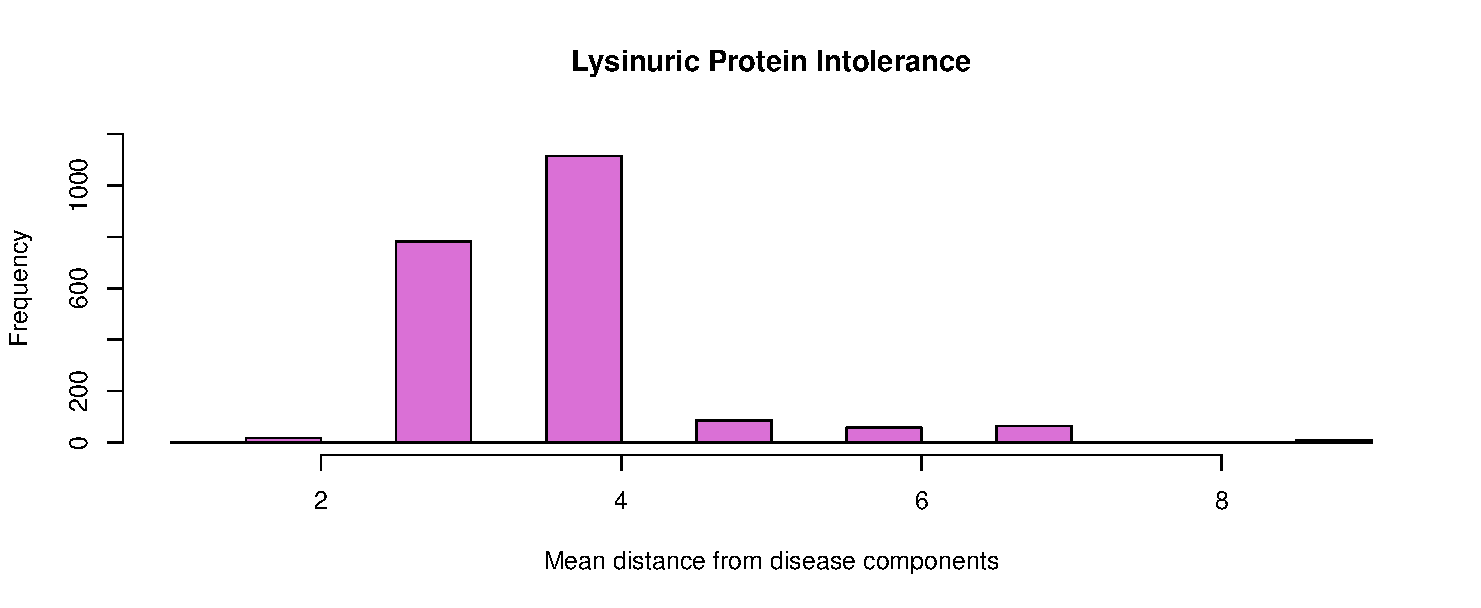
\includegraphics[scale=0.25]{Images/Lisinuric Protein Intolerance.pdf}
         \caption{LPI}
         \label{fig:Lisinuric}
     \end{subfigure}
     \hfill
     \begin{subfigure}[b]{0.3\textwidth}
         \centering
         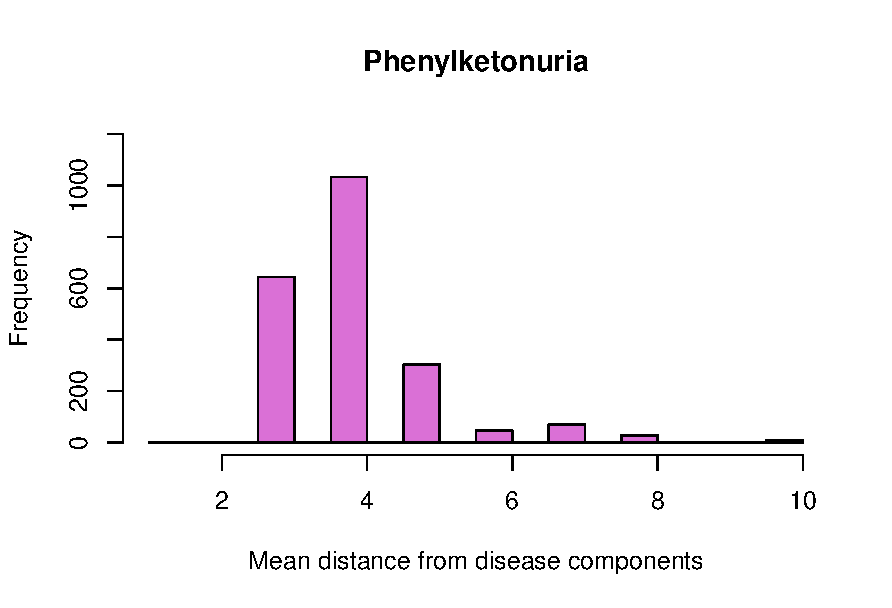
\includegraphics[scale=0.25]{Images/Phenylketonuria.pdf}
         \caption{Phenylketonuria}
         \label{fig:Phenylketonuria}
     \end{subfigure}
     \hfill
     \begin{subfigure}[b]{0.3\textwidth}
         \centering
         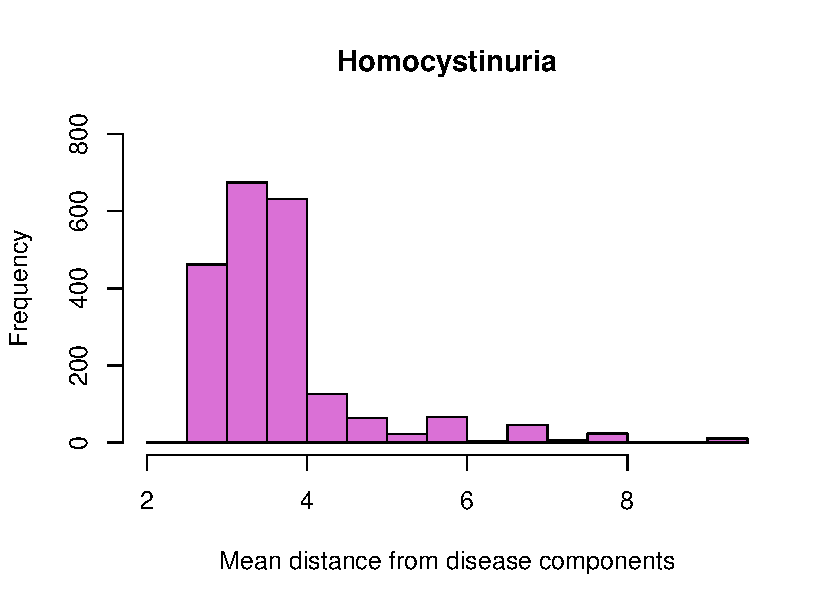
\includegraphics[scale=0.25]{Images/Homocystinuria.pdf}
         \caption{Homocystinuria}
         \label{fig:Homocystinuria}
     \end{subfigure}
     \hfill
     \begin{subfigure}[b]{0.3\textwidth}
         \centering
         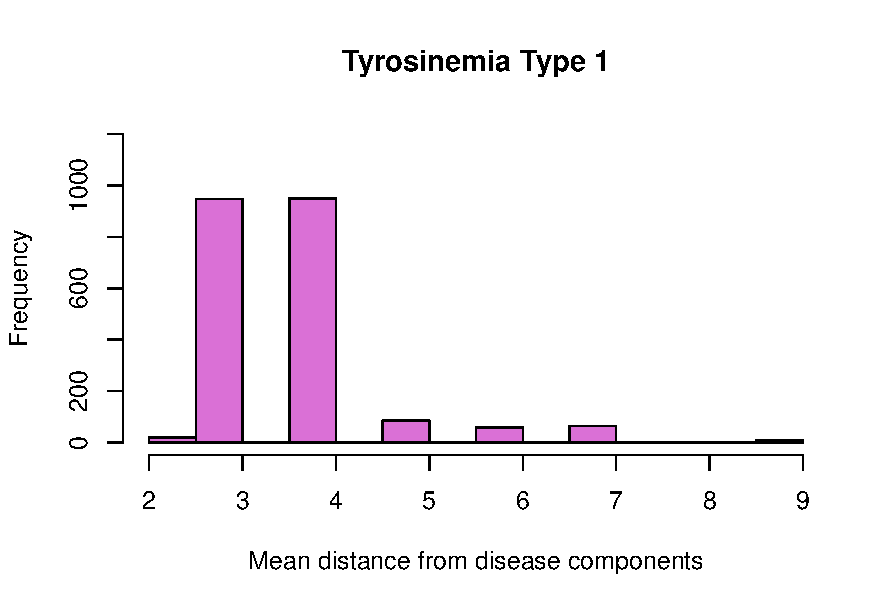
\includegraphics[scale=0.25]{Images/Tyrosinemia Type I.pdf}
         \caption{Tyrosinemia Type I}
         \label{fig:Tyrosinemia Type I}
     \end{subfigure}
     \hfill
     \begin{subfigure}[b]{0.3\textwidth}
         \centering
         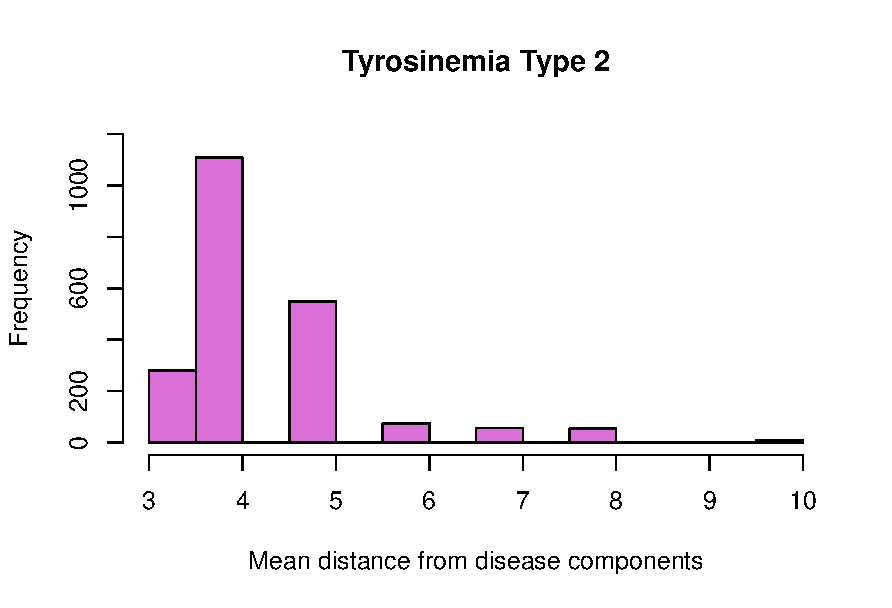
\includegraphics[scale=0.25]{Images/Tyrosinemia Type II.pdf}
         \caption{Tyrosinemia Type II}
         \label{fig:Tyrosinemia Type II}
     \end{subfigure}
     \hfill
     \begin{subfigure}[b]{0.3\textwidth}
         \centering
         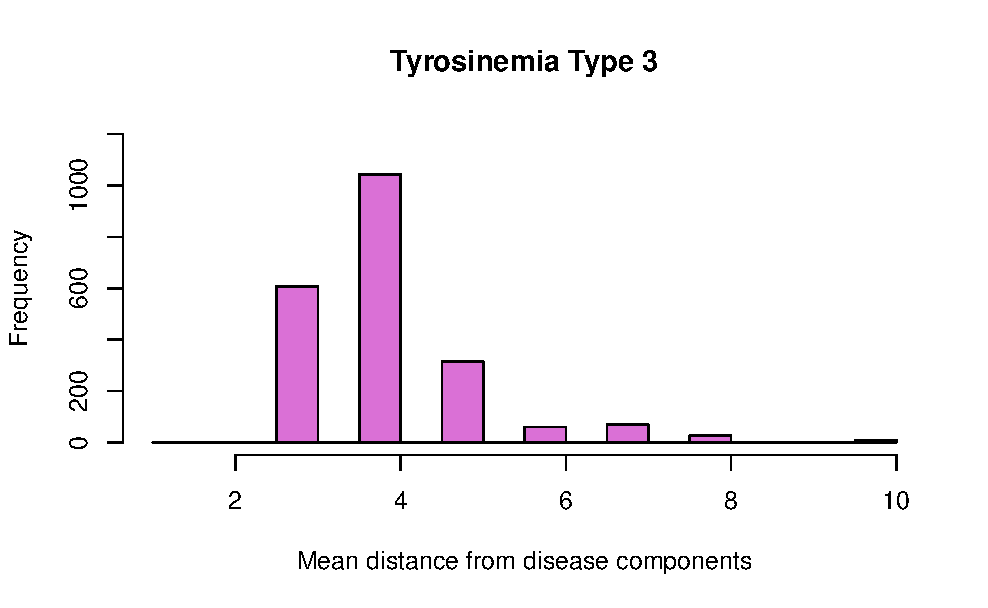
\includegraphics[scale=0.25]{Images/Tyrosinemia Type III.pdf}
         \caption{Tyrosinemia Type III}
         \label{fig:Tyrosinemia Type III}
     \end{subfigure}
     \hfill
     \begin{subfigure}[b]{0.3\textwidth}
         \centering
         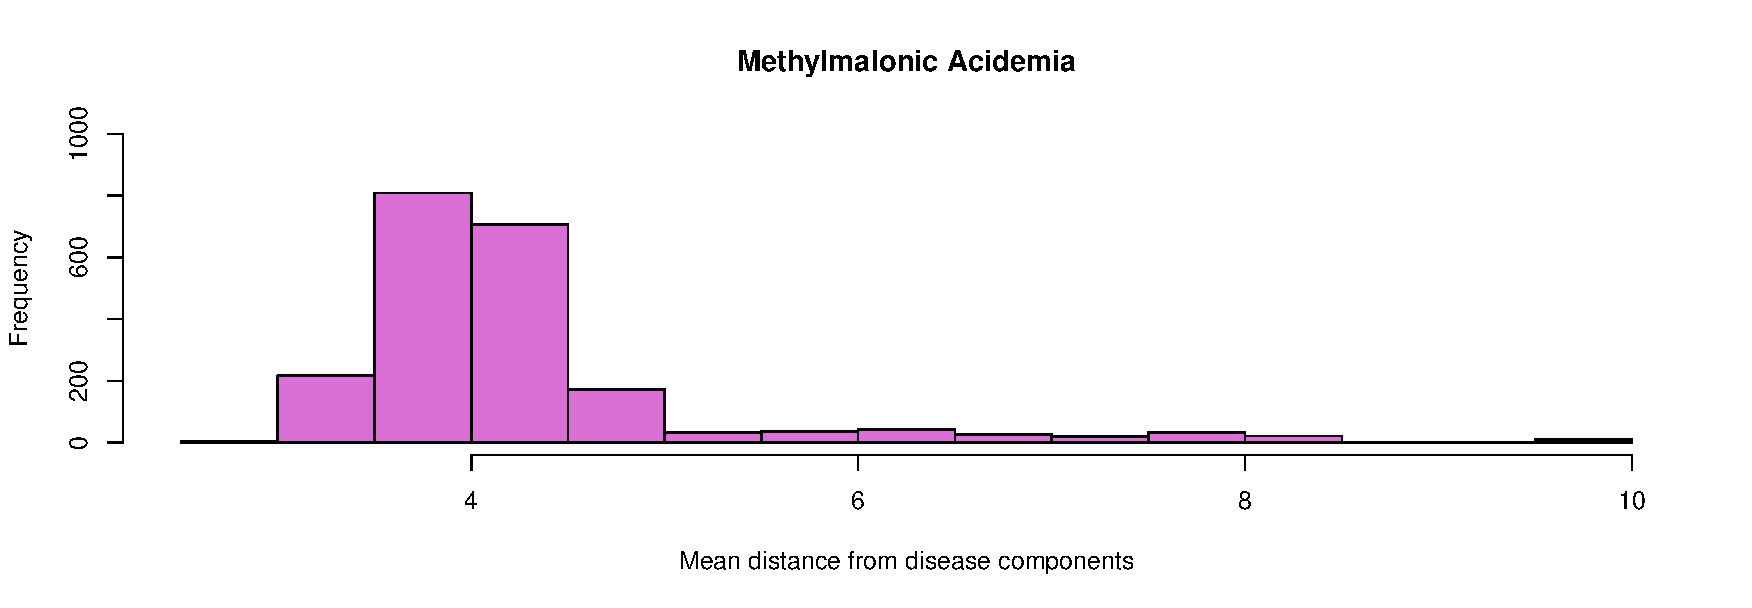
\includegraphics[scale=0.25]{Images/Methylmalonic Acidemia.pdf}
         \caption{Methylmalonic A.}
         \label{fig:Methylmalonic Acidemia}
     \end{subfigure}
     \hfill
     \begin{subfigure}[b]{0.3\textwidth}
         \centering
         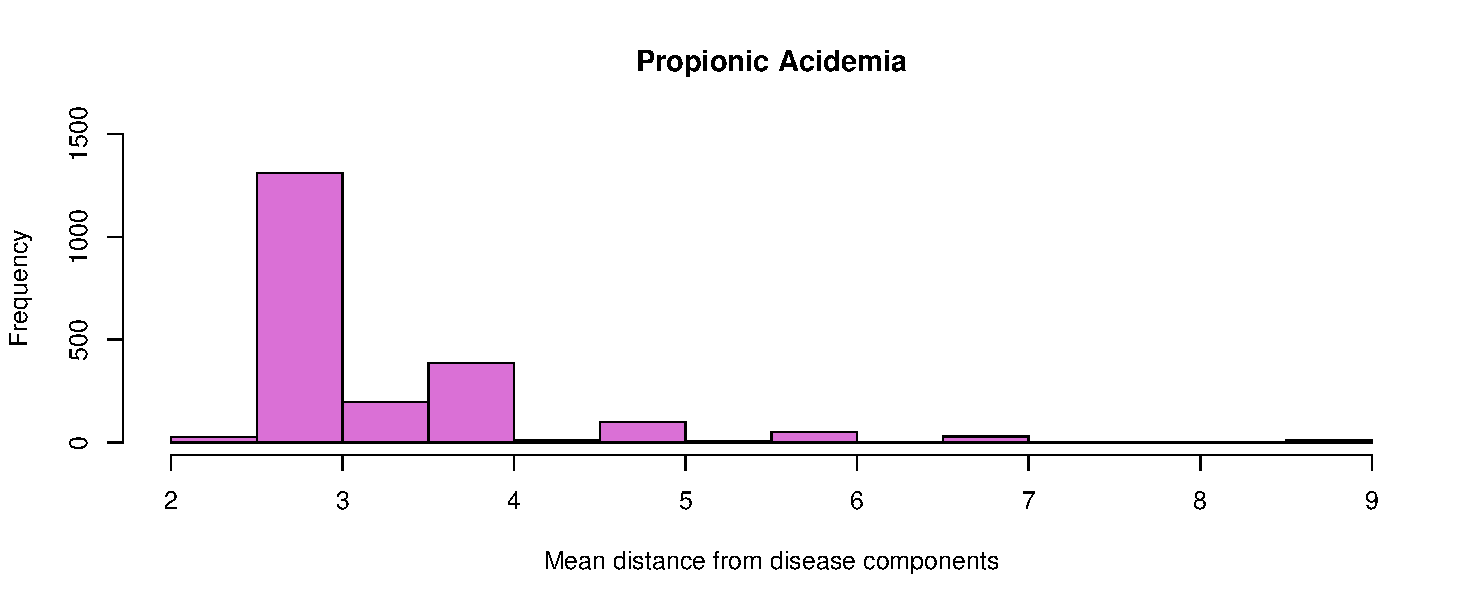
\includegraphics[scale=0.25]{Images/Propionic Acidemia.pdf}
         \caption{Propionic Acidemia}
         \label{fig:Propionic Acidemia}
     \end{subfigure}
     \hfill
     \begin{subfigure}[b]{0.3\textwidth}
         \centering
         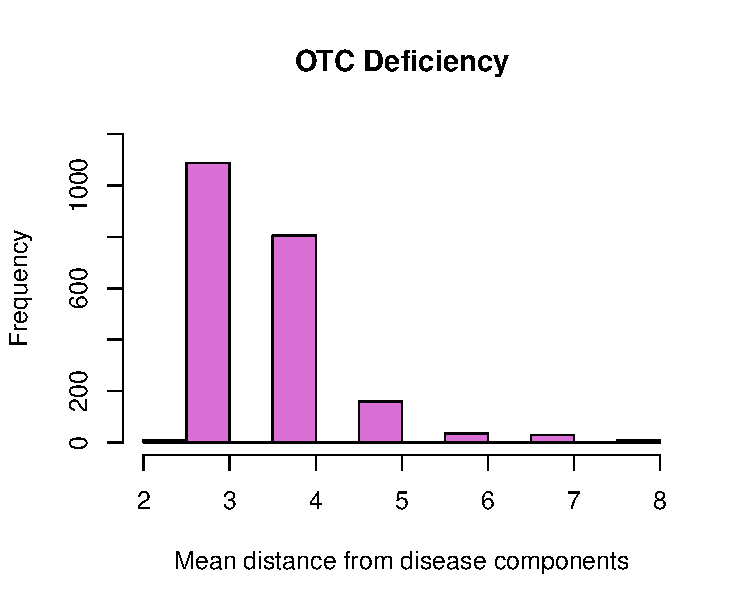
\includegraphics[scale=0.25]{Images/OTC Deficiency.pdf}
         \caption{OTC Deficiency}
         \label{fig:OTC}
     \end{subfigure}
     \hfill
      \begin{subfigure}[b]{0.3\textwidth}
         \centering
         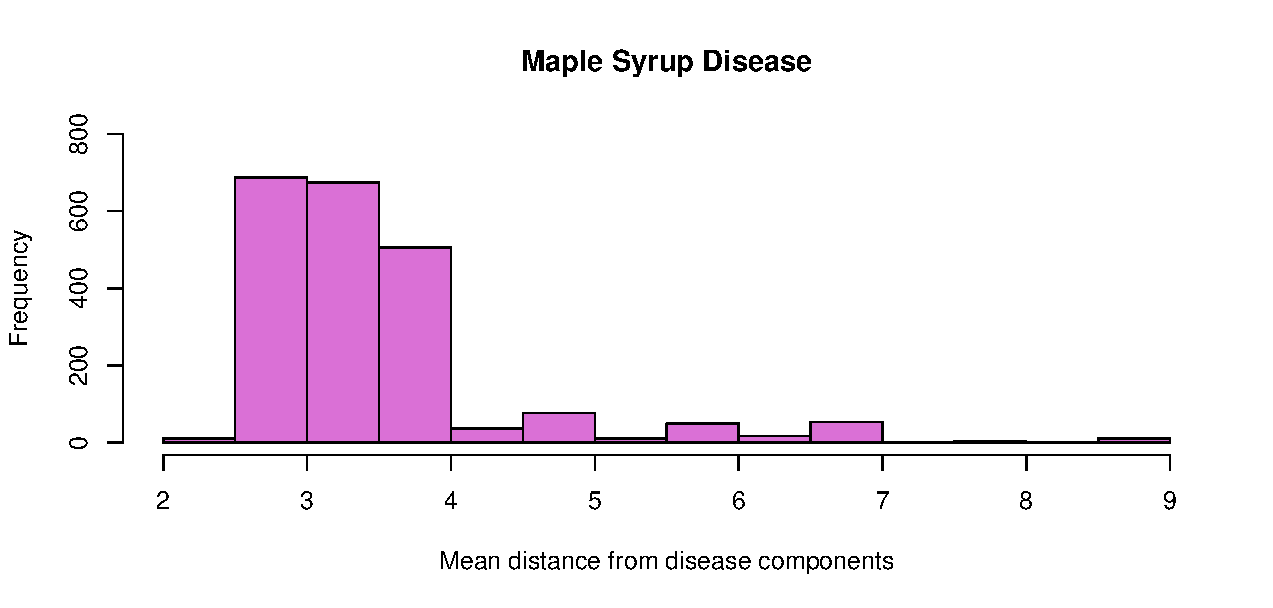
\includegraphics[scale=0.25]{Images/Maple Syrup Disease.pdf}
         \caption{Maple Syrup Disease}
         \label{fig:Maple Syrup}
     \end{subfigure}
     \hfill
     \begin{subfigure}[b]{0.3\textwidth}
         \centering
         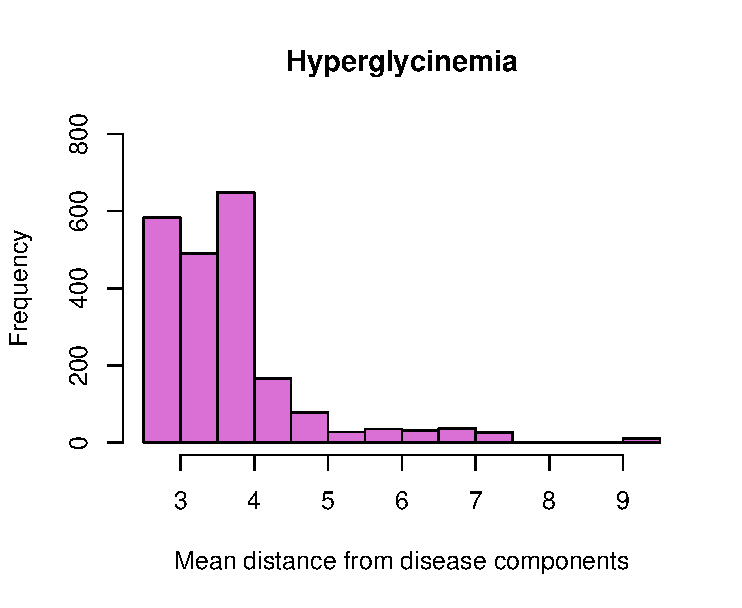
\includegraphics[scale=0.25]{Images/Hyperglycinemia.pdf}
         \caption{Hyperglycinemia}
         \label{fig:Hyperglycinemia}
     \end{subfigure}
     \hfill
     \begin{subfigure}[b]{0.3\textwidth}
         \centering
         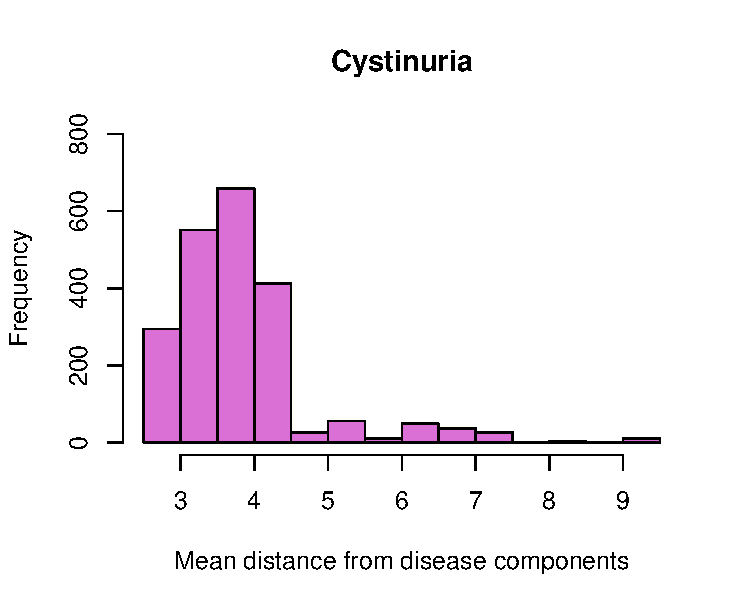
\includegraphics[scale=0.25]{Images/Cystinuria.pdf}
         \caption{Cystinuria}
         \label{fig:Cystinuria}
     \end{subfigure}
     \hfill
    \caption{Drugs mean distances frequency distribution for each disease's ranking}
    \label{fig:results}
\end{figure}
\FloatBarrier
\chapter{Conclusions}

By selecting pathways related to disorders of amino acid metabolism from ``Reactome'' and enriching the generated graphs with interactions related to the drugs, healthy metabolic processes and the main biological processes of the human organism related to the former via ``Biogrid'', it was possible to produce a ranking of the 2220 drugs obtained from ``DrugBank'' for each of the 12 identified metabolic diseases. 
An interesting and valuable feature of the resulting rankings is the distribution of the percentages of drugs per rank. In fact, thanks to the bell curve of distribution, the drugs which achieved the best ranks in most are for most of the diseases in very low percentage considered the total number of 2220 drugs,

\section{Future Plans}
During the development, as well as following the analysis of the results, several insights emerged that could be taken into consideration for future approaches and directions for the project.

Thanks to its modular and extensible nature, in fact, the implementation would lend itself to the application of analyses to other sets of drugs, taken for instance from other databases, representing other drug categories or even simply from the mentioned (and also ignored for the purposes of the project) ``all.csv" file from ``DrugBank".

It would also be relevant to perform ranking even with less basic algorithms, potentially even disengaging from the use of distances as a ranking parameter, exploring instead factors such as flow or approaches similar to the ``PageRank" algorithm.

Finally, of even greater importance would be the submission of the results obtained from the ranking to experts in Biology and Metabolic Diseases, in order to obtain a practical and effective test of the system's performance, as well as fulfilling the essential purpose of research and the project's goals in the field of drugs repurposing.

% Mostra bibliografia
\printbibliography[heading=bibintoc]

%``"
\end{document}

